\documentclass[11pt]{article} 
\usepackage[english]{babel}
\usepackage[utf8]{inputenc}
\usepackage[margin=0.5in]{geometry}
\usepackage{amsmath}
\usepackage{amsthm}
\usepackage{amsfonts}
\usepackage{amssymb}
\usepackage[usenames,dvipsnames]{xcolor}
\usepackage{graphicx}
\usepackage[siunitx]{circuitikz}
\usepackage{tikz}
\usepackage[colorinlistoftodos, color=orange!50]{todonotes}
\usepackage{hyperref}
\usepackage[numbers, square]{natbib}
\usepackage{fancybox}
\usepackage{epsfig}
\usepackage{soul}
\usepackage[framemethod=tikz]{mdframed}
\usepackage[shortlabels]{enumitem}
\usepackage[version=4]{mhchem}
\usepackage{multicol}
\usepackage{algorithm}
\usepackage[noend]{algpseudocode}


\usepackage{mathtools}
\usepackage{comment}
\usepackage{enumitem}
\usepackage[utf8]{inputenc}
%\usepackage[linesnumbered,ruled,vlined]{algorithm2e}
\usepackage{listings}
\usepackage{color}
\usepackage[numbers]{natbib}
\usepackage{subfiles}
\usepackage{tkz-berge}


\newtheorem{prop}{Proposition}[section]
\newtheorem{thm}{Theorem}[section]
\newtheorem{lemma}{Lemma}[section]
\newtheorem{cor}{Corollary}[prop]

\theoremstyle{definition}
\newtheorem{definition}{Definition}

\theoremstyle{definition}
\newtheorem{required}{Problem}
\newtheorem*{requiredHC}{Problem HC}

\theoremstyle{definition}
\newtheorem{ex}{Example}


\setlength{\marginparwidth}{3.4cm}
%#########################################################

%To use symbols for footnotes
\renewcommand*{\thefootnote}{\fnsymbol{footnote}}
%To change footnotes back to numbers uncomment the following line
%\renewcommand*{\thefootnote}{\arabic{footnote}}

% Enable this command to adjust line spacing for inline math equations.
% \everymath{\displaystyle}

% _______ _____ _______ _      ______ 
%|__   __|_   _|__   __| |    |  ____|
%   | |    | |    | |  | |    | |__   
%   | |    | |    | |  | |    |  __|  
%   | |   _| |_   | |  | |____| |____ 
%   |_|  |_____|  |_|  |______|______|
%%%%%%%%%%%%%%%%%%%%%%%%%%%%%%%%%%%%%%%

\title{
\normalfont \normalsize 
\textsc{CSCI 3104 Spring 2023 \\ 
Instructors: Chandra Kanth Nagesh and Prof. Ryan Layer} \\
[10pt] 
\rule{\linewidth}{0.5pt} \\[6pt] 
\huge Quiz 19 Standard 19 -- (Divide \& Conquer) MergeSort \\
\rule{\linewidth}{2pt}  \\[10pt]
}
%\author{Your Name}
\date{}

\begin{document}
\definecolor {processblue}{cmyk}{0.96,0,0,0}
\definecolor{processred}{rgb}{200, 0, 0}
\definecolor{processgreen}{rgb}{0, 255, 0}
\DeclareGraphicsExtensions{.png}
\DeclareGraphicsExtensions{.gif}
\DeclareGraphicsExtensions{.jpg}

\maketitle


%%%%%%%%%%%%%%%%%%%%%%%%%
%%%%%%%%%%%%%%%%%%%%%%%%%%
%%%%%%%%%%FILL IN YOUR NAME%%%%%%%
%%%%%%%%%%AND STUDENT ID%%%%%%%%
%%%%%%%%%%%%%%%%%%%%%%%%%%
\noindent
Due Date \dotfill TODO \\
Name \dotfill \textbf{Blake Raphael} \\
Student ID \dotfill \textbf{109752312} \\
Quiz Code (enter in Canvas to get access to the LaTeX template) \dotfill \textbf{IKJOP}


\tableofcontents

\section*{Instructions}
\addcontentsline{toc}{section}{Instructions}
 \begin{itemize}
	\item You may either type your work using this template, or you may handwrite your work and embed it as an image in this template. \textbf{If you choose to handwrite your work, the image must be legible, and oriented so that we do not have to rotate our screens to grade your work.} We have included some helpful LaTeX commands for including and rotating images commented out near the end of the LaTeX template.
	\item You should submit your work through the \textbf{class Gradescope page} only. Please submit one PDF file, compiled using this \LaTeX \ template.
	\item You may not need a full page for your solutions; pagebreaks are there to help Gradescope automatically find where each problem is. Even if you do not attempt every problem, please submit this document with no fewer pages than the blank template (or Gradescope has issues with it).

	\item You \textbf{may not collaborate with other students}. \textbf{Copying from any source is an Honor Code violation. Furthermore, all submissions must be in your own words and reflect your understanding of the material.} If there is any confusion about this policy, it is your responsibility to clarify before the due date. 

	\item Posting to \textbf{any} service including, but not limited to Chegg, Discord, Reddit, StackExchange, etc., for help on an assignment is a violation of the Honor Code.

	\item You \textbf{must} virtually sign the Honor Code (see Section \ref{HonorCode}). Failure to do so will result in your assignment not being graded.
\end{itemize}


\newpage
\section*{Honor Code (Make Sure to Virtually Sign)} \label{HonorCode}
\addcontentsline{toc}{section}{Honor Code (Make Sure to Virtually Sign)}
\hypertarget{HonorCode}{}

\begin{requiredHC}
\begin{itemize}
\item My submission is in my own words and reflects my understanding of the material.
\item Any collaborations and external sources have been clearly cited in this document.
\item I have not posted to external services including, but not limited to Chegg, Reddit, StackExchange, etc.
\item I have neither copied nor provided others solutions they can copy.
\end{itemize}

%\noindent In the specified region below, clearly indicate that you have upheld the Honor Code. Then type your name. 
\end{requiredHC}

\begin{proof}[Agreed (I agree to the above, Blake Raphael).]
%% Typing "I agree to the above," followed by your name is sufficient.
\end{proof}


\newpage
\setcounter{section}{18}
\section{Standard 19 -- (Divide \& Conquer) MergeSort (4 points)}

\setcounter{required}{18}
\begin{required} 
Consider a modified version of \textsc{MergeSort}, which divides the array into 6 (as equally-sized as possible) partitions (\textbf{Recall:} Standard \textsc{MergeSort} partitions the array into 2-equal sized sets). This variation of \textsc{MergeSort} is called the `k-way' \textsc{MergeSort}, where $k = 6$. Instead of dividing
the input array into two subarrays, `6-way' \textsc{MergeSort} divides the array into \textbf{six} subarrays, sorts them recursively, and then call a `6-way' \textsc{Merge} which combines six sorted arrays into one sorted array. (4 points)

Do the following \textbf{three} parts of the question.

\begin{enumerate}
\item \textbf{Write down} the number of comparisons that occur in the `6-way' \textsc{Merge} function, in the worst case. Assume we have six `M-element' arrays. (1 point) \\
(\textbf{Note:} In the worst case, a `2-way' \textsc{Merge} function performs $2M-1$ comparisons, where we assume to have two `M-element' arrays. \textbf{Donot} give a Big-O notation.)

\begin{proof}[Answer]
	The 6-way \textsc{Merge} function would perform $6M - 1$ comparisons at the worst case.\\
\end{proof}

\vspace{1in}

\item Now, with the the number of comparisons from part (1) \textbf{write down} the recurrence relation for the runtime of this modified version of `6-way' \textsc{MergeSort}. \textbf{Justify your recurrence relation in 1--2 sentences.} (1 point)
\begin{proof}[Answer]
% YOUR ANSWER HERE
\begin{align*}
	T(n) = \begin{cases}
		\Theta(1) & : n \leq 1, \\
		6T(n/6) + \Theta(n) & : n > 1.
	\end{cases}
\end{align*}

This is the recurrence relation because with each recursion, we break the array down 6 more times, which is $6 * n/6$.\\

\end{proof}

\vspace{1in}

\item Solve your recurrence relation from part (1), by any method you choose. \textbf{Show your work.}  Find a function $f(n)$ such that the runtime $T(n)$ is $T(n) = O(f(n))$. (2 points) \\
(\textbf{Further: } You need not show this work, but would a `6-way' \textsc{MergeSort} sort elements faster than `2-way' \textsc{MergeSort}.)

\begin{proof}[Answer]
% YOUR ANSWER HERE
Here we will use the tree method to solve the recurrence relation.\\

\begin{center}
	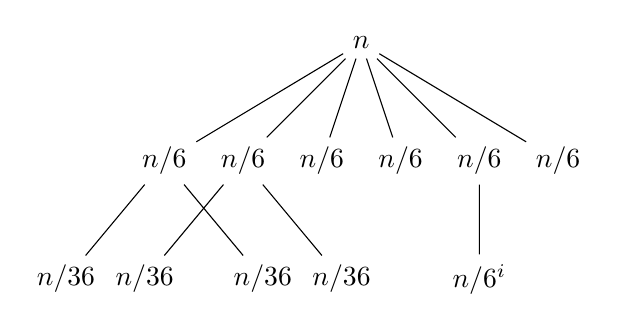
\begin{tikzpicture}
		\tikzstyle{level 1}=[sibling distance=10mm]
		\tikzstyle{level 2}=[sibling distance=25mm]
		\node {$n$}
		child {node {$n/6$}
			child {node{$n/36$}}
			child {node{$n/36$}}}
		child {node{$n/6$}
			child{node{$n/36$}}
			child{node{$n/36$}}}
		child {node{$n/6$}}
		child {node{$n/6$}}
		child {node{$n/6$}
			child {node{$n/6^i$}}}
		child {node{$n/6$}};
	\end{tikzpicture}\\
\end{center}

So we see that the non-recursive work at each level is $(n/6^i) * 6^i$.\\

We also hit our base case at $n/6^k \leq 1$ or $n \leq 6^k$. Solving for $k$, we get $k \leq \log_6(n)$.\\

So the total work performed by our 6-way mergesort is $\displaystyle\sum_{i=0} ^{\log_6(n)} n = n \cdot \log_6(n)$.\\

So we see that $T(n) \in \Theta(n\log(n))$.\\

A 6-way mergesort would not solve any faster than a 2-way mergesort. They have the same $\Theta$ runtimes.
\end{proof}

\vspace{1in}

\end{enumerate}

\end{required}

%%%%%%%%%%%%%%%%%%%%%%%%%%%%%%%%%%%%%%%%%%%%%%%%%%
\end{document} % NOTHING AFTER THIS LINE IS PART OF THE DOCUMENT



